\documentclass{article}
\usepackage{graphicx}
\usepackage[margin=1.5cm]{geometry}
\usepackage{amsmath}

\begin{document}

\title{Thursday Reading Assessment: Chapter 2-8, 2-10 through 2-12}
\author{Prof. Jordan C. Hanson}

\maketitle

\section{Hexadecimal and Other Number Systems}

\begin{enumerate}
\item Let $x_1 = FB17_{16}$, and $x_2 = 8A9D_{16}$.
\begin{enumerate}
\item What is $x_1$ in binary? \\ \vspace{1cm}
\item What is $x_2$ in decimal? \\ \vspace{1cm}
\end{enumerate}
\item Imagine a stream of binary digits coming through a serial line.  They are: $1001 ... 0001 ... 0001$.  If we know the bitstream is in binary coded decimal (BCD), what is the code being sent? \\ \vspace{1cm}
\item Which of the following is an \textit{invalid} BCD code?
\begin{itemize}
\item A: 0001
\item B: 0101
\item C: 1000
\item D: 1010
\end{itemize}
\item
\begin{figure}[hb]
\centering
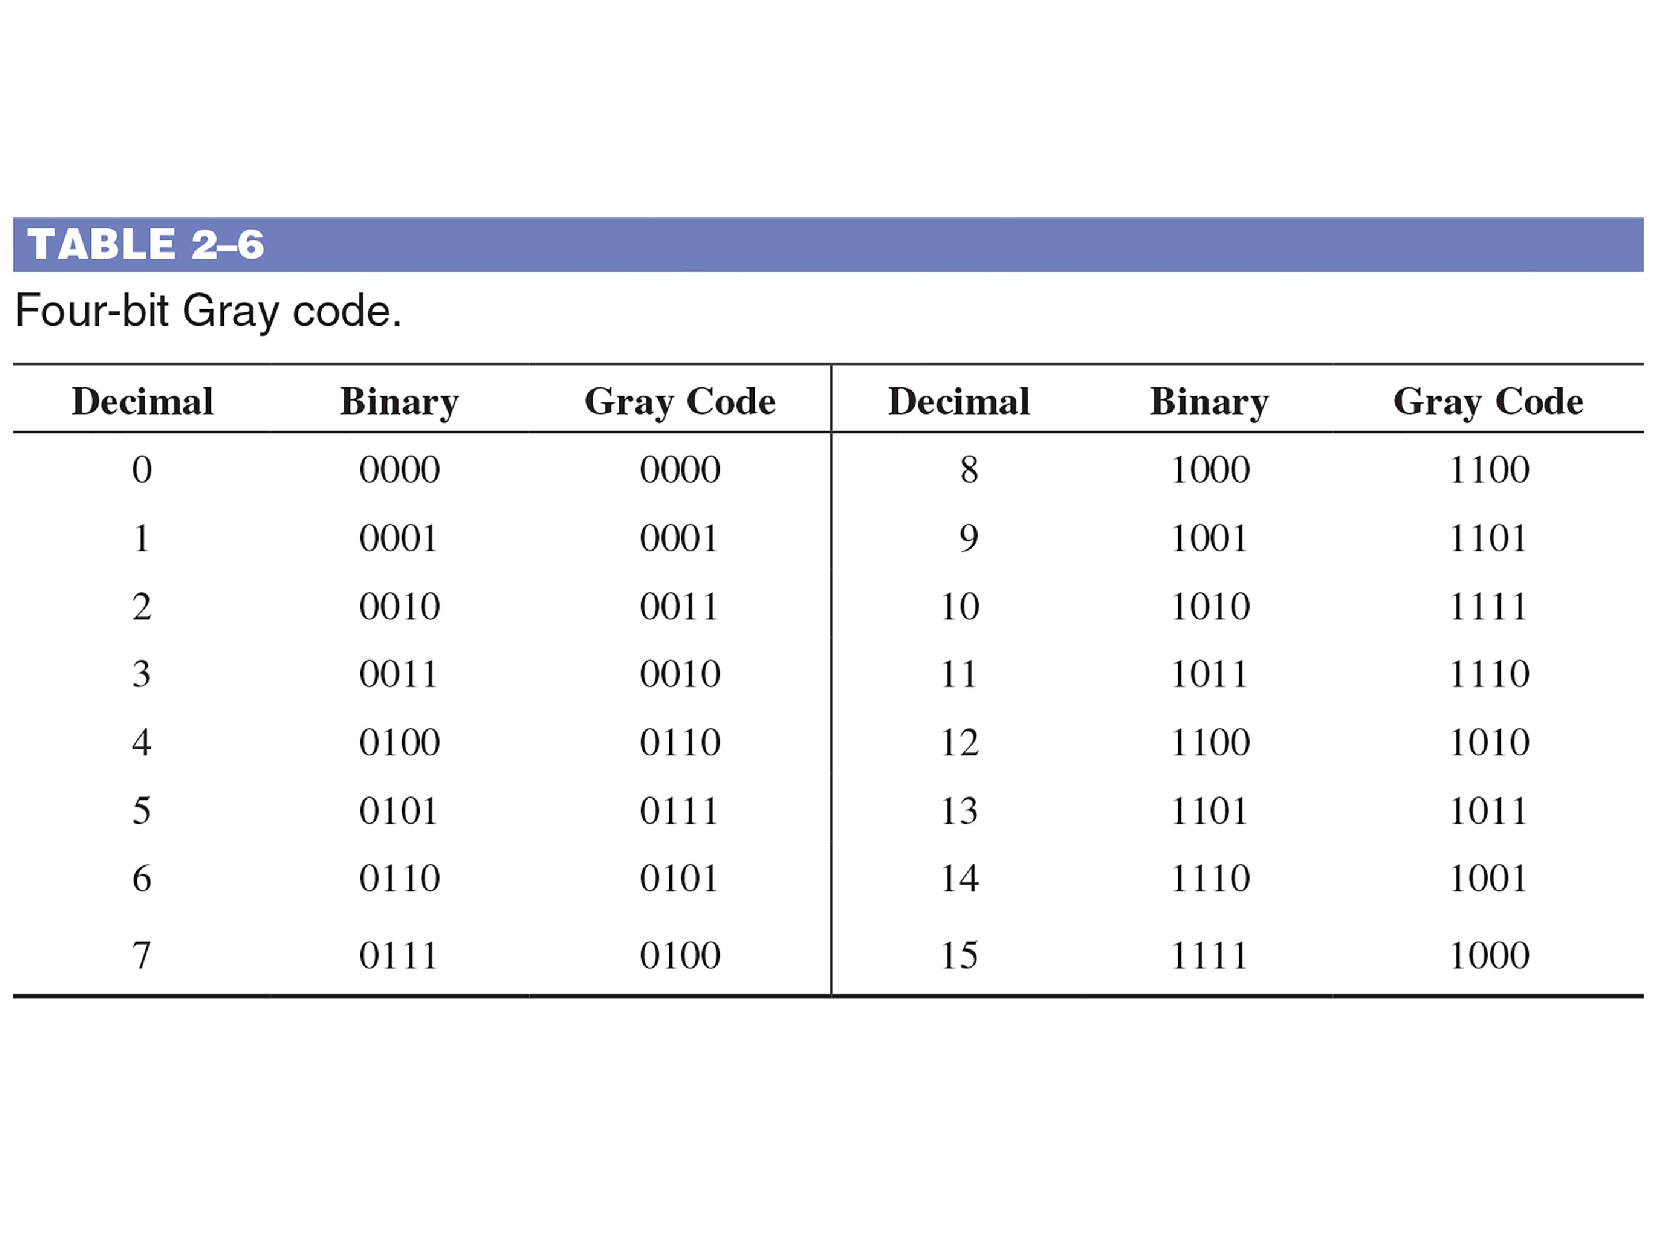
\includegraphics[width=0.45\textwidth]{gray.pdf}
\caption{\label{fig:gray} A four-bit binary gray code.}
\end{figure}
\item What property of the four-bit gray code in Fig. \ref{fig:gray} distinguishes it from straight binary counting?
\end{enumerate}

\end{document}
